%!TEX root = doc.tex
\documentclass[twoside,10pt,parskip=half,ngerman]{scrreprt}

%***********************************************************************
% include some libs
%***********************************************************************
\usepackage[utf8]{inputenc}
\usepackage{listings}
\usepackage{xcolor}
\usepackage{color}
\usepackage{fancyhdr}
\usepackage{rotating}
\usepackage{titlesec}
\usepackage{mathptmx}
\usepackage{amssymb} % checkmark
% \usepackage{helvet}
\usepackage[scaled]{uarial}
\renewcommand*\familydefault{\sfdefault} %% Only if the base font of the document is to be sans serif
\usepackage[T1]{fontenc}
\usepackage[ngerman]{babel}
\usepackage[pdfauthor={Nicolas Roos}, pdftitle={Projektarbeit im Seminar Mobile Netzwerke - Wifi basierte Aktionen (Android App)}, colorlinks=true,linkcolor=black,citecolor=black,plainpages=false]{hyperref}
\usepackage{textcomp}
\usepackage[squaren]{SIunits}
\usepackage{graphicx}
\usepackage{url}
\usepackage{geometry}
\usepackage[absolute]{textpos}
\usepackage{makeidx}
\usepackage{colortbl}
\usepackage{pdflscape}
\usepackage{pdfpages}
\usepackage{tabularx}
\usepackage{lmodern}
\usepackage{longtable}
\usepackage{array}
\usepackage{float}
\usepackage{scrhack}
\usepackage{wallpaper} %\ThisTileWallPaper{}
\usepackage[super,square]{natbib} %für BibTeX Literaturverzeichnis
\usepackage{packages/usecases}
% Glossar
\usepackage{footnote}
\makesavenoteenv{description}
\usepackage[acronym,section=section]{glossaries}
\renewcommand*{\glsentryfmt}{\ifglsused{\glslabel}{\glsentryname{\glslabel}}{\glsentrydesc{\glslabel}\space(\glsentryname{\glslabel})}}
\makeglossaries

%***********************************************************************
% various styles
%***********************************************************************

%create index
\makeindex

%define pagestyle
\pagestyle{fancy}

%use sans-serif font
%\renewcommand{\familydefault}{\sfdefault}

%define page margin
\geometry{a4paper, top=30mm, left=30mm, right=30mm, bottom=30mm,headsep=10mm,footskip=10mm}

%textpos parameter
\setlength{\TPHorizModule}{30mm}
\setlength{\TPVertModule}{\TPHorizModule}
\textblockorigin{10mm}{10mm} % start everything near the top-left corner
\setlength{\parindent}{0pt}

%horizontal lines for titlepage
\newcommand{\HRule}{\rule{\linewidth}{0.5mm}}

%reference to source items inlc source number
\newcommand{\srcref}[1]{\nameref{src:#1} \cite{#1}}

%header / footer
\renewcommand{\headrulewidth}{0.3pt}
\renewcommand{\footrulewidth}{0.3pt}

\fancyhead[LO,RE]{} %clear headings for contents
\fancyhead[RO,LE]{\nouppercase{\rightmark}} %right odd pages and left even pages
\fancyhead[LO,RE]{\MakeUppercase{\leftmark}} %left odd pages and right even pages
\fancyfoot[LE,RO]{\thepage} %page numbering
\fancyfoot[C]{} %clear centered page numbering

%define some colors
\definecolor{gray}{rgb}{0.95,0.95,0.95}
\definecolor{darkgray}{rgb}{0.4,0.4,0.4}
%listing colors
\definecolor{lgray}{RGB}{250,250,250}
\definecolor{lgreen}{RGB}{63,127,95}
\definecolor{lred}{RGB}{127,0,85}
\definecolor{lblue}{RGB}{42,0,255}

%***********************************************************************
% listing
%***********************************************************************

\lstset{
		basicstyle=\small\ttfamily,
		frame=single,
		numbers=left,
		numberstyle=\tiny,
		%firstnumber=auto,
		numberblanklines=true,
		captionpos=b,
		extendedchars=true,
		float=ht,
		showtabs=false,
		tabsize=2,
		showspaces=false,
		showstringspaces=false,
		breaklines=true,
		%prebreak=\Righttorque,
		backgroundcolor=\color{lgray},
		keywordstyle=\color{lred}\bfseries,
		commentstyle=\color{lgreen}\ttfamily,
%		morekeywords={printstr, printhexln},
		stringstyle=\color{lblue},
		xleftmargin=0.5cm,
		xrightmargin=0.5cm
}

\lstloadlanguages{[Sharp]C}
%\lstdefinestyle{sharpc}{language=[Sharp]C, frame=lr} %, rulecolor=\color{blue!80!black}

%\lstdefinelanguage{xc}{
%     keywords={printstr, printhexln, attributes, class, classend, do, empty, endif, endwhile, fail, function, functionend, if, implements, in, inherit, inout, not, of, operations, out, return, set, then, types, while, use},
%     keywordstyle=\color{lred}\bfseries,
%     ndkeywords={},
%     ndkeywordstyle=\color{yellow}\bfseries,
%     identifierstyle=\color{black},
%     sensitive=false,
%     comment=[l]{//},
%     commentstyle=\color{lgreen}\ttfamily,
%     string=[l]{"},
%     stringstyle=\color{lblue}\ttfamily
%  }


\begin{document}
%!TEX root = ../doc.tex
\newglossaryentry{zhaw}{name=ZHAW,description=Zürcher Hochschule für Angewandte Wissenschaften}

\bibliographystyle{plainnat}

\title{Projektarbeit im Seminar Mobile Netzwerke - Wifi basierte Aktionen (Android App)} % In header.tex nachtragen
\author{Nicolas Roos}

%!TEX root = ../doc.tex
\begin{titlepage}

% Logo
\ThisTileWallPaper{\paperwidth}{\paperheight}{images/logos/SoE.pdf} % {images/logos/*.pdf}

\begin{minipage}[b]{0.117\textwidth}
\hskip 0.05cm
\end{minipage}
\begin{minipage}[b]{0.91\textwidth}
\begin{tiny}.\end{tiny}\vskip 2.8cm
	{\huge

	% Projekt Name (max. 2 Zeilen)
	\textbf{\underline{Bachelor-/Projektarbeit}}\\
	\textbf{\underline{FS14 Studiengang Informatik}}\\

	% Projekt Titel (max. 4 Zeilen)
	Titel der Arbeit
	\vskip 0.5cm}

	\begin{minipage}[b]{0.27\textwidth}
	\hrule\vskip 0.5cm
		\textbf{Autoren}\\
		\\
	\end{minipage}
	\begin{minipage}[b]{0.03\textwidth}
	\hskip 0.5cm
	\end{minipage}
	\begin{minipage}[b]{0.7\textwidth}
	\hrule\vskip 0.5cm
		Vorname Name\\
		Vorname Name\\
	\end{minipage}

	\begin{minipage}[b]{0.27\textwidth}
	\hrule\vskip 0.5cm
		\textbf{Hauptbetreuung}\\
		\\
	\end{minipage}
	\begin{minipage}[b]{0.03\textwidth}
	\hskip 0.5cm
	\end{minipage}
	\begin{minipage}[b]{0.7\textwidth}
	\hrule\vskip 0.5cm
		Vorname Name\\
		Vorname Name\\
	\end{minipage}

	\begin{minipage}[b]{0.27\textwidth}
	\hrule\vskip 0.5cm
		\textbf{Nebenbetreuung}\\
		\\
	\end{minipage}
	\begin{minipage}[b]{0.03\textwidth}
	\hskip 0.5cm
	\end{minipage}
	\begin{minipage}[b]{0.7\textwidth}
	\hrule\vskip 0.5cm
		Vorname Name\\
		Vorname Name\\
	\end{minipage}

	\begin{minipage}[b]{0.27\textwidth}
	\hrule\vskip 0.5cm
		\textbf{Industriepartner}\\
		\\
	\end{minipage}
	\begin{minipage}[b]{0.03\textwidth}
	\hskip 0.5cm
	\end{minipage}
	\begin{minipage}[b]{0.7\textwidth}
	\hrule\vskip 0.5cm
		Firmenname\\
		\\
	\end{minipage}

	\begin{minipage}[b]{0.27\textwidth}
	\hrule\vskip 0.5cm
		\textbf{Externe Betreuung}\\
		\\
	\end{minipage}
	\begin{minipage}[b]{0.03\textwidth}
	\hskip 0.5cm
	\end{minipage}
	\begin{minipage}[b]{0.7\textwidth}
	\hrule\vskip 0.5cm
		Vorname Name\\
		Vorname Name\\
	\end{minipage}

	\begin{minipage}[b]{0.27\textwidth}
	\hrule\vskip 0.5cm
		\textbf{Datum}
	\end{minipage}
	\begin{minipage}[b]{0.03\textwidth}
	\hskip 0.5cm
	\end{minipage}
	\begin{minipage}[b]{0.7\textwidth}
	\hrule\vskip 0.5cm
		\today
	\end{minipage}
\end{minipage}
\vskip 0.5cm


\textcolor{darkgray}{
Bitte füllen Sie das Titelblatt aus und berücksichtigen Sie Folgendes:\\
 -> Bitte auf keinen Fall Schriftart und Schriftgrösse ändern. Text soll lediglich überschrieben werden!\\
 -> Bitte pro Tabellenzeile max. 4 Textzeilen!\\
\\
•	Titel: Fügen Sie Ihren Studiengang direkt nach dem Wort „Bachelorarbeit“ ein (max. 2 Zeilen).\\
•	Titel der Arbeit: Überschreiben Sie den Lauftext mit dem Titel Ihrer Arbeit (max. 4 Zeilen).\\
•	Autoren: Tragen Sie Ihre Vor- und Nachnamen ein (alphabetisch nach Name).\\
•	Betreuer: Tragen Sie Ihren Betreuer / Ihre Betreuer ein (alphabetisch nach Name).\\
•	Ohne Nebenbetreuung, Industriepartner oder externe Betreuung, ganze Tabellenzeile löschen.\\
•	Am Schluss löschen Sie den ganzen Beschrieb (grau) und speichern das Dokument als pdf. ab.
}

\end{titlepage}

\setcounter{page}{1}
%!TEX root = ../doc.tex
\thispagestyle{empty}
\chapter*{Abstract}
\label{sec:abstract}
This is a paper about the development of a proof of concept for an university project. The goal was to implement an Android app that can execute certain predefined tasks when reaching or leaving a wifi network. Another part of this paper is the analysis of the density of wifis in cities as big as Zürich. The app has implemented all the requirments defined in chapter \ref{sec:anforderungsanalyse} and is available on github.com\footnote{Github repository: \url{https://github.com/roosnic1/wifi_action}}.

%\includepdf{images/Erklaerung_PA.pdf} % Entsprechendes auskommentieren
% \includepdf{images/Erklaerung_BA.pdf}
% \newpage

%Inhaltsverzeichnis
\tableofcontents
\newpage

%\textbf{}
%\setcounter{page}{1}
%\pagenumbering{arabic}

%!TEX root = ../doc.tex
\chapter{Einleitung}
\label{sec:Einleitung}

\section{Ausgangslage}
\label{sec:Ausgangslage}

Viele Mobile Apps erlauben dem Benutzer/der Benutzerin Aktionen auszuführen, wenn ein bestimmter geographischer Punkt bzw. Bereich erreicht oder verlassen wird. Aufgrund des erhöhten Batterieverbrauchs bei aktivem GPS Dienst und der hohen Anzahl von Wireless LANs in den meisten grösseren Städten, erscheint es sinnvoll diese Benutzerdefinierten Aktionen auch beim erreichen oder verlassen eines Wireless LANs auszuführen.

\section{Ziel der Arbeit}
\label{sec:zielderarbeit}
Das Ziel der Arbeit ist eine Prototyp App für Android zu entwickeln, welche dem Benutzer bzw. der Benutzerin erlaubt Aktionen zu definieren, welche beim Verbinden bzw. Verlassen von Wireless LANs ausgeführt werden. Unter Aktionen wird zum Beispiel das ändern des Benachrichtigungsmodus (Lautlos, Haptisches Feedback, Klingelton) oder die Aktivierung bzw. Deaktivierung des Bluetooth Verbindung verstanden.

\section{Aufgabenstellung}
\label{sec:aufgabenstellung}
\begin{itemize}
  \item Recherche über bereits existierende Apps und die Möglichkeiten des Android SDK.
  \item Erstellen einer kleine Anforderungsanalyse.
  \item Entwicklung eines Prototyp der Android App.
  \item Erstellen eines Entwicklungsbericht.
  \item Erstellen einer Präsentation.
\end{itemize}

\section{Erwartete Resultate}
\label{sec:erwarteteresultate}
\begin{itemize}
  \item Abgeschlossene Recherche
  \item Fertige Anforderungsanalyse mit Anforderungen und Tests
  \item Getesteter und funktionierender Prototyp
  \item Entwicklungsbericht
  \item Präsentation
\end{itemize}
%!TEX root = ../doc.tex
\chapter{Wireless LAN Grundlagen}
\label{sec:TheoretischeGrundlagen}

\section{Definition}
Ein Wireless LAN ist ein Funknetz welches die Übertragung von Daten von einem Endgerät (Computer, Handy, usw.) durch die Luft zu einem Access Point erlaubt. Die meisten Wireless LAN Standards sind in der IEEE-802.11 Familie beschrieben und werden von den meisten neueren Geärten, welche mit Wireless LAN ausgestattet sind, unterstützt. Das Wireless LAN ersetzt in vielen Bereichen das LAN bzw. das Kabel, welches früher für die Verbindung mit einem LAN benötigt wurde.

\section{Technisch}
Die Primäre Funktion eines Wireless LAN Access Point ist das herstellen einer Verbindung zwischen 802.11 Wireless LAN und 802.3 Ethernet Datenverkehr. Ein Access Point sendet in einem Intervall (ca. 10 mal pro Sekunde) seine Verbindungsinformationen an alle Wireless Geräte in seiner Reichweite. Die Informationen bestehen aus folgenden Bestandteilen.
\begin{itemize}
\item Der Netzwerkname - SSID
\item Die Liste der unterstützten Übertragungsraten
\item Die Art der Verschlüsselung
\end{itemize}
Mit diesen Angaben kann ein Wireless Gerät mit dem korrekten Passwort sofern notwendig eine Verbindung mit dem Access Point herstellen. Wireless LAN Access Points operieren auf der Sicherungsschicht (Schicht 2) des OSI Modell. Auf der gleichen OSI Schicht arbeiten auch herkömmliche LANS. Weil beide Standards auf der gleichen Schicht arbeiten, können sie auch ohne weiteres miteinander Kommunizieren. \newline{}
Ein Access Point kann nur innerhalb eines bestimmten Radius Senden und Empfangen. Für ein grösseres Wireless LAN Netzwerk müssen mehrere Access Points verwendet werden. Diese haben dieselbe SSID aber eine eindeutige BSS. In der Abbildung \ref{fig:bssap} wird das Prinzip dargestellt. Mehrere BSS mit derselben SSID sind ein ESS.
\begin{figure}[ht]
	\centering
	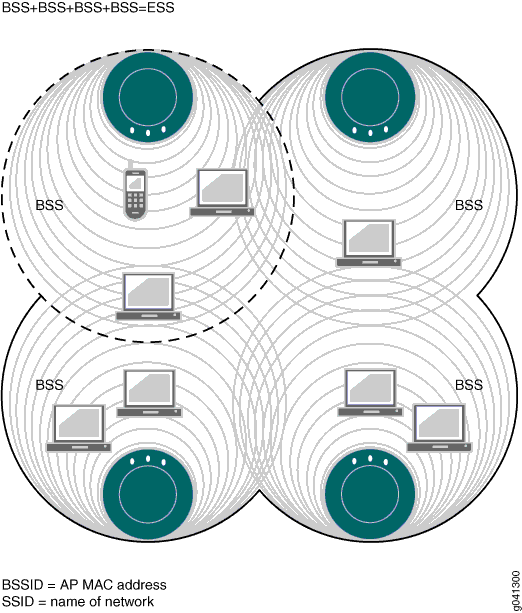
\includegraphics[width=0.8\textwidth]{images/bssssid.png}
	\caption{Jeder Access Point hat eine eigene BSS}
	\label{fig:bssap}
\end{figure}


\section{Verbreitung}
Das Schweizer Bundesamt für Statistik hat im Februar 2011 Daten zur Internetnutzung der Schweiz erhoben und kam zum Schluss, dass 58\% der Schweizer Haushalte über ein Wireless LAN verfügen\citep[S. 8]{bfs.internet.2011}. Zusätzlich werden in den grösseren Städten in den öffentlichen Gebäuden (Bahnhof, Flughafen usw.) sowie in vielen Cafes Wireless LANs Gratis oder gegen Bezahlung angeboten. Zahlen zu der Dichte von Wireless LAN in Europäischen Städten scheint es nicht zu geben oder sind sehr schwierig zu finden. Für die Benutzbarkeit der zu erstellenden App ist das Aufkommen von Wireless LANs in den Städten ein kritischer Faktor.

\subsection{Experiment Zürich}
Um Einschätzen zu können wie viele Access Point in einer Stadt zu finden sind, wurde ein kleines Experiment durch geführt. Mit der Android App WiFi Tracker\citep{google.play.wifitracker} werden alle Wireless LAN Netzwerke in welchen sich das Mobiltelefon befindet, mit den aktuellen GPS Koordinaten gespeichert. Mit dem Fahrrad und dem Mobiltelefon wurde eine Strecke von ca. 3.1 Kilometern durch den Zürcher Kreis 4 abgefahren. Die Aufgezeichneten Daten bringen erstaunliches zum Vorschein.
\begin{figure}[ht]
	\centering
	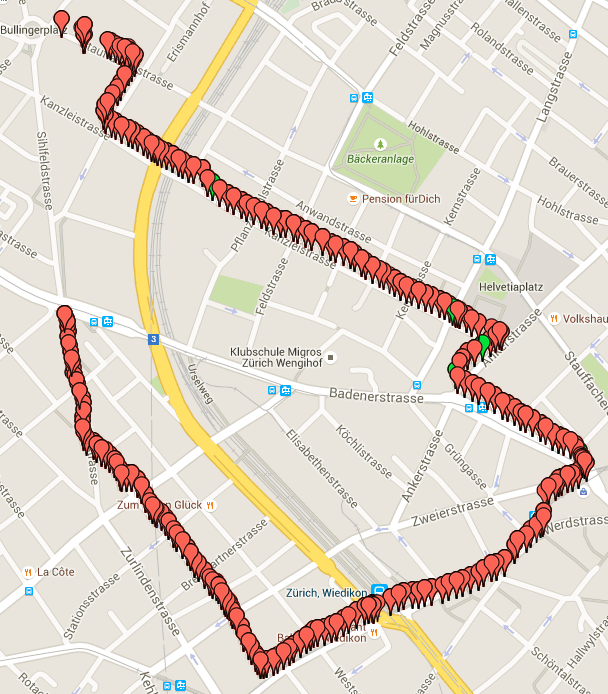
\includegraphics[width=0.8\textwidth]{images/wifikreis4.png}
	\caption{Wireless LANs gemesen mit WiFi Tracker im Zürcher Kreis 4}
	\label{fig:wifikreis4}
\end{figure}
Auf der Strecke wurden 2253 unterschiedliche Access Points gemessen welche in der Abbildung \ref{fig:wifikreis4} visuell dargestellt sind. Das heisst durchschnittlich ist nach 1.37 Meter ein neuer Access Point zu finden. Diese Zahlen müssen natürlich ein wenig relativiert werden da die 2253 Access Points nicht zwingend auch eigene Wireless LAN Netzwerke sind. Wie oben beschrieben können mehrere Access Points mit der selben SSID zu einem Wireless LAN Netzwerk gehören. Zusätzlich ist der Zürcher Kreis 4 nicht ein repräsentatives Gebiet, welches auf den Rest von Zürich oder andere Städte schliessen lässt. Trotzdem lassen diese Zahlen auf eine grosse Wireless LAN Dichte in Schweizerischen Städten deuten.


 % (2. Theoretische Grundlagen)
%!TEX root = ../doc.tex
\chapter{Recherche}
\label{sec:recherche}

\section{Apps}
Die Recherche im Google Play Store hat ergeben dass einige Apps existieren, welche ähnliche Funktionalität wie die in dieser Arbeit zu entwickelnde App auch anbietet. Im folgenden werden 4 Apps genauer analysiert.

\subsection{Tasker}
Tasker\citep{google.play.tasker} ist eine App welche auf den ersten Blick alles anbietet. Die App kann beinahe auf jegliche Statusänderung reagieren. Sei es GPS Koordinaten oder eine SMS mit einem bestimmten Kennwort. Es erlaubt auch das Ausführen von Aktionen beim Verbinden oder Verlassen eines Wireless LANs. Die App wirkt aber auf den ersten Blick sehr umständlich und Kostet 3.99 CHF.

\subsection{Task Center}
Task Center\citep{google.play.taskcenter} scheint der schlanke Bruder von Tasker zu sein. Die App kann gratis genutzt werden und ist mit In-App Käufen auch Werbefrei. Bei Task Center wird die Aktion jedoch nur bei Veränderung des Wireless LAN Verbingunsstatus ausgeführt. Dabei spielt der Netzwerkname bzw. die SSID keine Rolle.

\subsection{NFC Actions}
NFC Actions\citep{google.play.nfcactions} hat ein sehr ähnliches Prinzip wie die zu entwickelnde App aber führt diese beim erkennen eines NFC Tags aus. Dabei können AKtionen wie Bluetooth Ein oder Ausschalten oder das anrufen einer Telefonnummer ausgeführt werden. Zusätzlich lassen sich eigene NFC Tags schreiben welche dann bestimmte Aktionen auslösen.

\subsection{Trigger}
Trigger\citep{google.play.trigger} ist die App welche dem in dieser Arbeit beschriebenen Konzept am nähsten kommt. Aktionen können beim Verbinden oder Verlassen von Wireless LANs ausgeführt werden. Das gleiche gilt auch für ads erreichen von GPS Koordinaten, NFC Tags und Bluetooth Netzwerke. Die App ist sehr umfangreich und hatte beim Testen mehrere Fehler sowie Abstürze.

\subsection{Fazit}
Die 3 analysierten Apps sowie die anderen welche bei der Recherche zum Vorschein kamen bieten einen ähnlichen Funktionsumfang an, wie die App welche im Rahmen dieser Arbeit erstellt werden soll. Jedoch zeigen alle Apps gewisse Defizite auf welche die Entwicklung einer neuen App rechtfertigen. Einige Apps sind so umfangreich dass sie nicht mehr intuitiv zu bedienen sind andere wiederum lassen nur einen sehr beschränken Auslöser zu.


\section{Android SDK}
Bei der Entwicklung soll besonders auf die Energiesparsamkeit der App geachtet werden. Das Konzept ist nicht neu und kann spielend einfach mit einer bereits existierenden App, welche Aktionen beim erreichen bestimmte GPS Koordinaten ausführt, umgesetzt werden. Jedoch verbrauchen solche Apps sehr viel Energie und können daher unter Umständen am entsprechenden Ort statt der Ausgeführten Aktion nur noch einen Schwarzen Bildschirm anzeigen. Diese soll bei der Ausführung der zu entwickelnden App nicht passieren. Daher soll die App nur aktiv werden wenn das System eine änderung des Wireless LAN Status erkannt hat. Dies verhindert dass die App in regelmässigen Intervallen den Status selber überprüfen muss. Zusätzlich muss beachtet werden dass beim Erreichen bzw. Verlassen eines Wireless LANs das Mobiltelefon meist nicht aktiv im Gebrauch ist. Daher muss die Aktion im Hintergrund ausgeführt werden können. Das Android Software Developer Kit bietet dafür einige Tools und APIs zur Verfügung, welche im folgenden genauer erläutert werden.

\subsection{BroadcastReceiver}
Ein BroadcastReceiver reagiert auf einen definierten Intent (Aktion) welcher vom Android System oder von anderen Applikationen ausgelöst wurde. Es lässt sich einen BroadcastReceiver erstellen welcher mit einem Filter wie \glqq android.net.conn.CONNECTIVITY\_CHANGE\grqq{} auf alle Verbindungswechsel reagieren kann. Das Auslesen der aktuellen Verbindungsinformationen wird in Abbildung \ref{fig:verbindungsinfo} dargestellt. Mit diesen Informationen lässt sich der Wechseln von Wireless LANs leicht erkennen.

\begin{figure}[ht]
\centering
\begin{subfigure}[b]{0.8\textwidth}
  \centering
  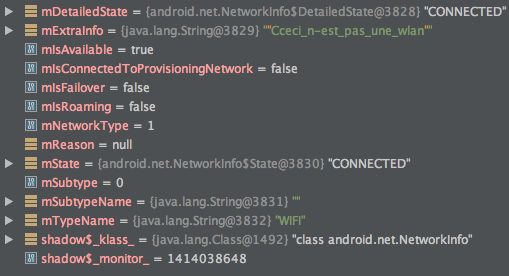
\includegraphics[width=1\linewidth]{images/debugwifi.png}
  \caption{Verbindung mit Wifi}
  \label{fig:sub1}
\end{subfigure}

\begin{subfigure}[b]{0.8\textwidth}
  \centering
  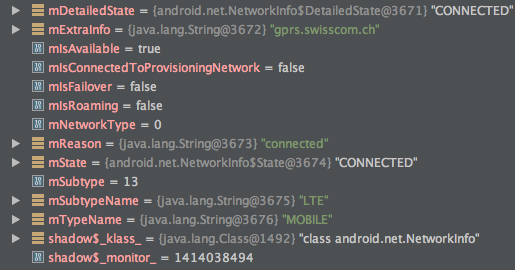
\includegraphics[width=1\linewidth]{images/debugnowifi.png}
  \caption{Verbindung ohne Wifi}
  \label{fig:sub2}
\end{subfigure}
\caption{Debug Informationen aus Android Studio}
\label{fig:verbindungsinfo}
\end{figure}


\subsection{IntentService}
Ein IntentService ist einen Android Komponente welche es erlaubt etwas in einem eigenen Thread auszuführen. Der Main Thread wird dadurch nicht gestört bzw. er wird nicht einmal benötigt, was das Ausführen bei inaktivem Mobiltelefon erlaubt. Weil der IntentService aber zur App gehört, kann auf die gemeinsamen Daten zugegriffen werden. Dadurch ist gewährleistet dass definierte Aktionen vom IntentService ausgeführt werden können.

\subsection{Aktionen/Tasks}
Die Ausführung der verfügbaren Aktionen wie z.B. das aktivieren bzw. deaktivieren des Bluetooth Statuses muss jeweils einzeln analysiert und umgesetzt werden. Gewisse Aktionen sind mit dem Android Software Developement Kit einfach umzusetzten andere wie das ein oder ausschalten des GPS Moduls nicht möglich. Android verlangt eine bewusste Interaktion des Benutzers wenn es um das verändern des GPS Status geht. Daher werden für diesen Prototypen eine limitierte Anzahl von Aktionen zur Verfügung stehen.
%!TEX root = ../doc.tex
\chapter{Anforderungsanalyse}
\label{sec:anforderungsanalyse}

\section{Use Cases}
Für die bessere Lesbarkeit werden in den Use Cases die folgenden Felder weg gelassen, weil sie immer den selben Wert haben.
\begin{usecase}
\addtitle{UC-000}{-}
\additemizedfield{Autoren}{
	\item (immer) Nicolas Roos
}
\additemizedfield{Quelle}{
	\item (immer) Nicolas Roos
}
\additemizedfield{Verantwortlicher}{
	\item (immer) Nicolas Roos
}

\end{usecase}

\newpage{}
\addcontentsline{toc}{subsection}{UC-001 Aktion definieren}
\begin{usecase}
\addtitle{UC-001}{Aktion definieren}
\addfield{Priorität}{Zwingend}
\addfield{Kritikalität}{Hoch}
\addfield{Beschreibung}{Der Benutzer kann eine Aktion für das erreichen bzw. verlassen eines bestimmten Wireless LANs definieren}
\addfield{Auslösendes Ereignis}{Der Benutzer erstellt eine neue Aktion}
\addfield{Akteure}{Benutzer}
\addfield{Vorbedingungen}{-}
\addfield{Nachbedingungen}{-}
\addfield{Ergebnis}{Eine gespeicherte Aktion}
\addscenario{Hauptszenario}{
	\item Der Benutzer erstellt eine neue Aktion.
	\item Der Benutzer wählt für die Aktion ein bestimmtes bekanntes Wireless LAN aus.
	\item Der Benutzer wählt wann die Aktion ausgeführt wird.
	\item Der Benutzer gibt noch zusätzliche Parameter ein.
	\item Die App speichert die Aktion.
}
\addfield{Alternativszenarien}{-}
%\addscenario{Alternativszenarien}{
%	\item Job wird über API gestartet...
%}
\addfield{Ausnahmeszenarien}{-}
%\addscenario{Ausnahmeszenarien}{\item ...}
\addfield{Qualitäten}{-}
\end{usecase}

\newpage{}
\addcontentsline{toc}{subsection}{UC-002 Aktion ausführen}
\begin{usecase}
\addtitle{UC-002}{Aktion ausführen}
\addfield{Priorität}{Zwingend}
\addfield{Kritikalität}{Hoch}
\addfield{Beschreibung}{Das System kann beim erreichen bzw. verlassen eines bestimmten Wireless LANs die definierte Aktion ausführen}
\addfield{Auslösendes Ereignis}{Die App erhält eine Meldung vom Android System}
\addfield{Akteure}{App}
\addfield{Vorbedingungen}{Die App läuft im Vordergrund oder Hintergrund und hat die Möglichkeit Systemmeldungen zu bekommen}
\addfield{Nachbedingungen}{-}
\addfield{Ergebnis}{Eine ausgeführte Aktion}
\addscenario{Hauptszenario}{
	\item Die App bekommt eine Meldung über die Änderung des Wireless LANs Status
	\item Die App überprüft ob für die Kombination (SSID und erreichen bzw. verlassen) eine Aktion vorhanden ist
	\item Die App führt die Aktion aus und Loggt das Ereignis
}
\addfield{Alternativszenarien}{-}
%\addscenario{Alternativszenarien}{
%	\item Job wird über API gestartet...
%}
\addfield{Ausnahmeszenarien}{-}
%\addscenario{Ausnahmeszenarien}{\item ...}
\addfield{Qualitäten}{-}
\end{usecase}


\newpage{}
\section{Funktionale Anforderungen}
\label{sec:funktionaleanforderungen}
%!TEX root = ../doc.tex
\chapter{Umsetzung des Prototyps}
\label{sec:umsetzung}

\section{Vorbereitung}
Für die Entwicklung des Prototypen wird Android Studio Version 1.2 von Google verwendet. Android Studio baut auf der freien Version von IntelliJ IDEA auf und verfügt daher über sehr viele nützliche Entwicklerwerkzeuge. Für die Versionskontrolle des Quellecodes wird Git und eine Repository auf Github\footnote{Repository auf Github: \url{https://github.com/roosnic1/wifi_action}} verwendet. Für das Testen der App wird ein Android Mobiltelefon des Types Nexus 5 mit der Android Version 5.1 verwendet. Das Android Projekt wird mit der neusten Android SDK Version entwickelt. Das bedeutet die App funktioniert nur auf Mobiltelefonen mit der Android Verison 5.1 dafür können die neusten Funktionen vom SDK verwendet werden. Die Dokumentation bzw. der Entwicklerbericht wird in Sublime Text 3 mit \LaTeX{} geschrieben.

\section{Entwicklung}
Für die Umsetzung der App werden im wesentlichen Activities, für die Darstellungen und Interaktionen mit dem Benutzer, sowie ein Receiver und ein Service benötigt. Dazu kommen noch Adapters und Modelle mit welchen Daten in einer Datenbank bzw. in eine Datei serialisiert werden können. Die einzelnen Komponenten werden in diesem Kapitel beschrieben und auf wichtige Eigenschaften wird hingewiesen.

\subsection{Activities}
In Android repräsentieren Activities eine Benutzeroberfläche. Für die App wurden 3 Activities verwendet, welche mit ihren Verbindungen in der Abbildung \ref{fig:activities} dargestellt sind.

% MainActivity->ActionActivity: open
% note over ActionActivity: create Action
% ActionActivity->MainActivity: return Action
% MainActivity->Action List: save Action
% MainActivity->LogActivity: open
% note over LogActivity: show Logs
\begin{figure}[ht]
    \centering
    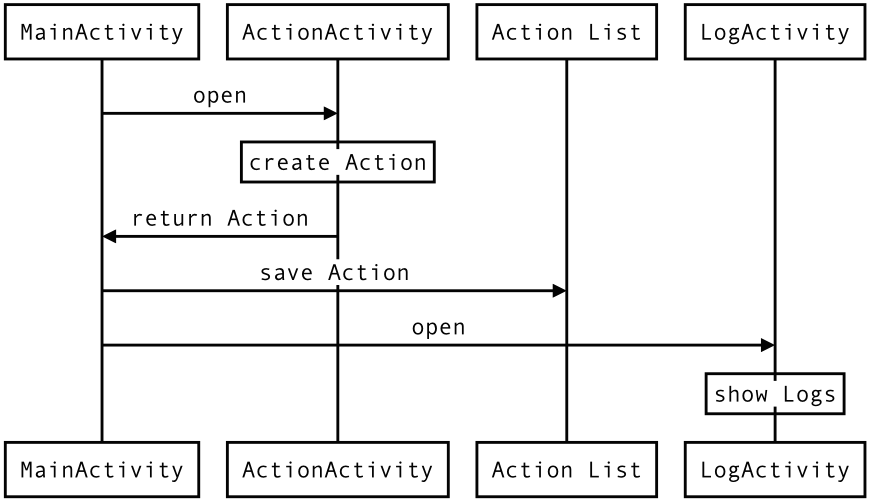
\includegraphics[width=0.7\textwidth]{images/activities.png}
    \caption{Sequenzdiagramm der verwendeten Activities}
    \label{fig:activities}
\end{figure}


\subsubsection{MainActivity}
Die MainActivity ist die Ansicht welche dem Benutzer angezeigt wird wenn der Benutzer die App startet. Wie in der Abbildung \ref{fig:mainactivity} beinhaltet die Activity in einer ListView alle bereits erstellten Aktionen und bietet über 2 Buttons die Transaktion zu der LogActivity und ActionActivity an.
\begin{figure}[ht]
	\centering
	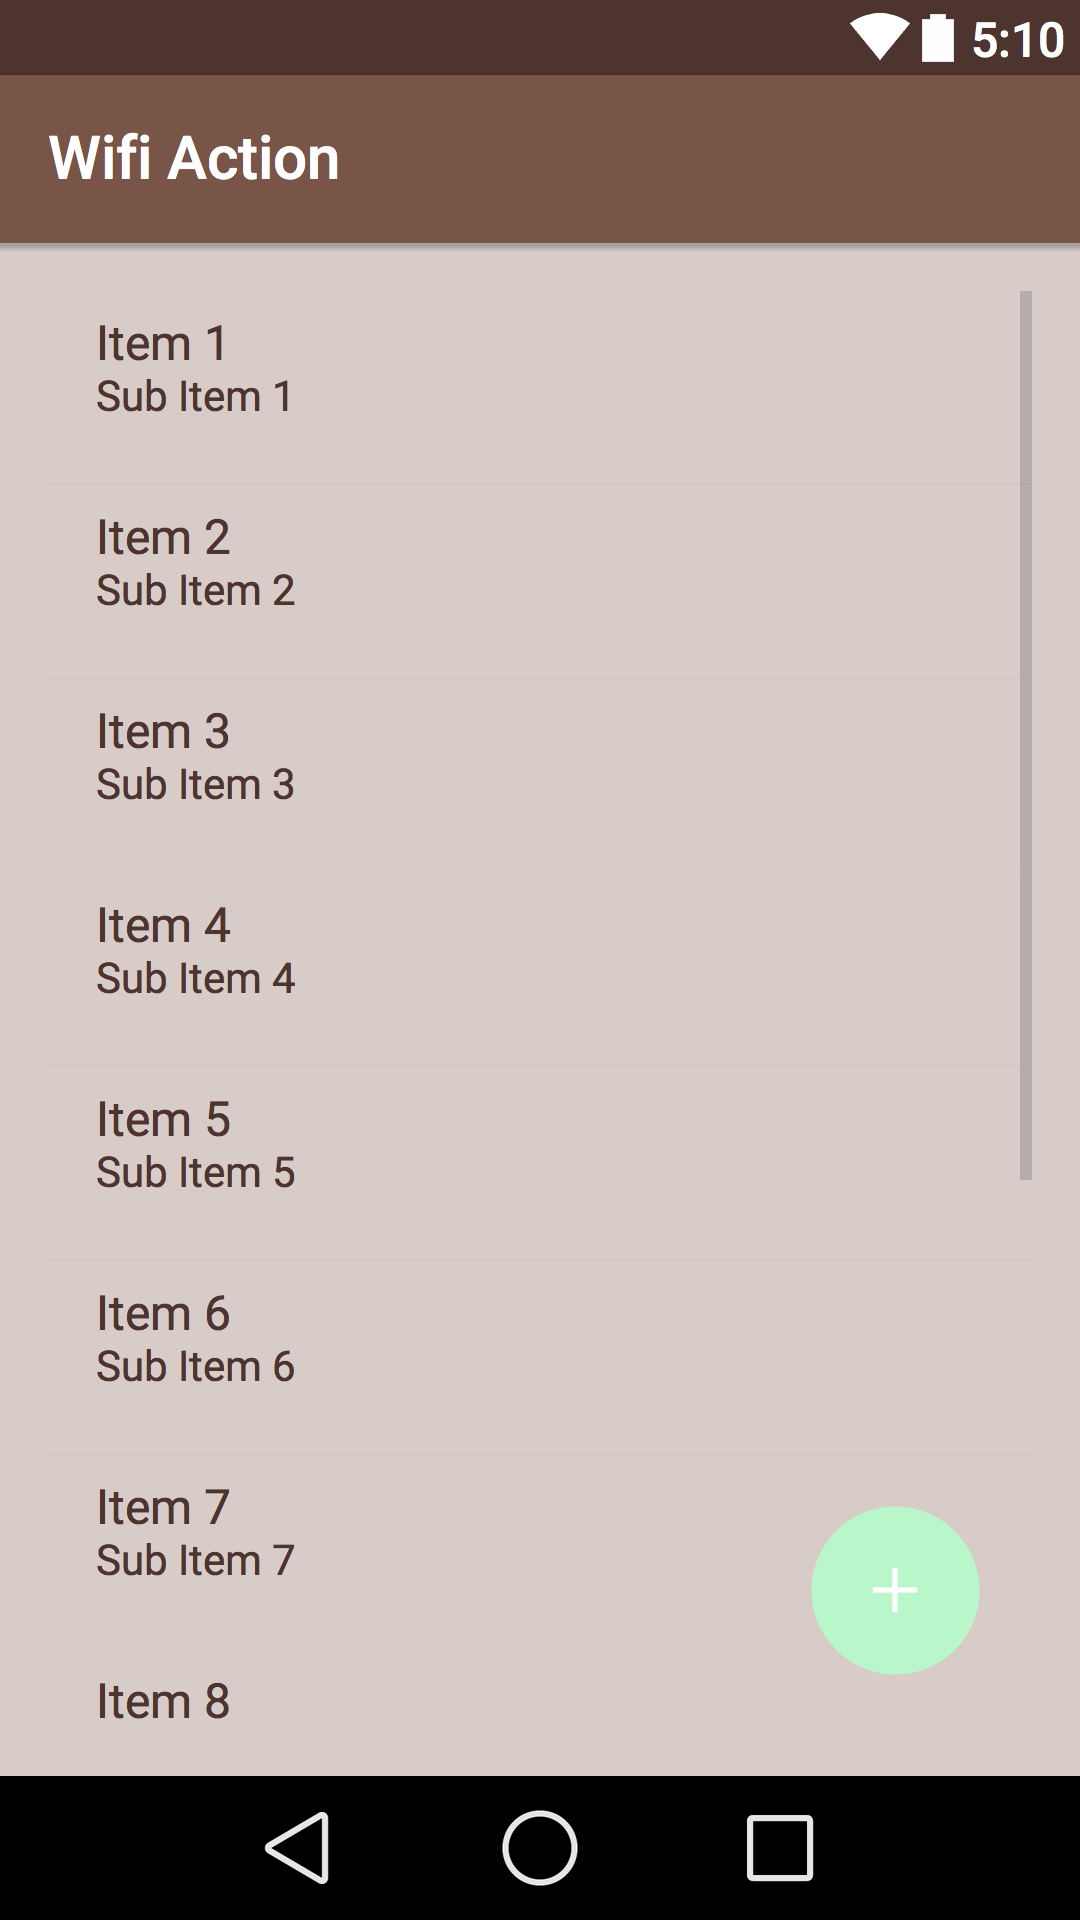
\includegraphics[width=0.4\textwidth]{images/mainactivity.png}
	\caption{Visuelle Repräsentation der MainActivity}
	\label{fig:mainactivity}
\end{figure}
Wenn die MainActivity gestartet wird, wird ein Asynchroner Job gestartet, welcher die serialisierten Aktion aus einer Datei lädt und anzeigt. Beim hinzufügen einer neuen Aktion werden alle Aktionen neu gespeichert damit keine verloren geht. Wenn eine Aktion in der Liste lange angeklickt wird, öffnet sich ein Kontext Menu, welches das löschen einer Aktion erlaubt. \\
Wird der Plus Button angeklickt werden alle bekannten Wireless LANs geladen und der ActionActivity übergeben. Das Laden der Wireless LANs ist mit Android einfach zu machen. \\
\begin{lstlisting}[language=Java]
	private ArrayList<Wifi> getKnownWifi() {
        WifiManager wifi = (WifiManager) getSystemService(Context.WIFI_SERVICE);
        List<WifiConfiguration> wifis = wifi.getConfiguredNetworks();
        ArrayList<Wifi> wifiList = new ArrayList<>();
        for(WifiConfiguration w : wifis) {
            wifiList.add(new Wifi(w.SSID,w.networkId););
        }
        return wifiList;
    }
\end{lstlisting}
Mit der Funktion getConfiguredNetworks() werden alle Wireless LANs ausgegeben mit denen das Mobiltelefon bereits eine Verbindung hatte.

\subsubsection{ActionActivity}
In der ActionActivity können neue Aktionen eingestellt und gespeichert werden. Im ersten Spinnerelement\footnote{In Android ist ein Spinnerelement eine Dropdown Liste} werden die Verfügbaren Aktionen angezeigt. Je nach Auswahl werden in der restlichen Ansicht unterschiedliche Felder angezeigt oder Versteckt. Deshalb überlagern sich gewisse Elemente in der Abbildung \ref{fig:actionctivity}. Im zweiten Spinnerelement werden die bekannten Wireless LANs angezeigt, welche von der MainActivity übergeben wurden. Die restlichen Elemente dienen der Einstellung der Aktion, welche über den Button \glqq Save\grqq{} gespeichert werden kann. Bei der Aktion Send SMS besteht die Möglichkeit eine Nummer aus dem Telefonbuch des Androidsystem auszuwählen. \\
\begin{lstlisting}[language=Java]
    public void onClick(View view) {
        Intent i = new Intent(Intent.ACTION_PICK, ContactsContract.CommonDataKinds.Phone.CONTENT_URI);
        startActivityForResult(i,REQUEST_CONTACTPICKER);
    }

    if(resultCode == RESULT_OK) {
        Uri contentUri = data.getData();
        Cursor cursor = getContentResolver().query(contentUri, null, null, null, null);
        cursor.moveToFirst();
        String number = cursor.getString(cursor.getColumnIndex(ContactsContract.CommonDataKinds.Phone.NUMBER));
        if(number.length() > 0) {
            etMessage3.setText(number);
        }
    }
\end{lstlisting}
Das Telefonbuch wird mit startActivityForResult gestartet und bei der Rückgabe wird der Eintrag aus dem Telefonbuch zurückgeben und ausgewertet. Dies hat den Vorteil dass die App nicht die Berechtigung zum lesen des Telefonbuches benötigt. Beim Drücken des \glqq Save\grqq{} Buttons werden die Daten zusammen gepackt und an die MainActivity zurück gegeben welche die Aktion speichert. \\
\begin{lstlisting}[language=Java]
-- ActionActivity.java -->
	Action a = new Action(etTitle.getText().toString(),((Wifi)spWifis.getSelectedItem()).getSsid(), at,cbOnConnect.isChecked(),cbOnLeave.isChecked());
	if(mActionType == 0) {
	    a.setStringParam1(etMessage3.getText().toString());
	} else {
	    a.setStringParam1(etMessage1.getText().toString());
	}
	a.setStringParam2(etMessage2.getText().toString());
	a.setBooleanParam1(swBoolean.isChecked());
	Intent i = new Intent();
	i.putExtra("ACTION",a);
	setResult(RESULT_OK, i);
	finish();
<----

-- MainActivity.java -->
	if(resultCode == RESULT_OK) {
		Action a = (Action) data.getSerializableExtra("ACTION");
		mActionList.add(a);
		actionAdapter.notifyDataSetChanged();
		saveActionList();
	}
<----
\end{lstlisting}
\begin{figure}[ht]
	\centering
	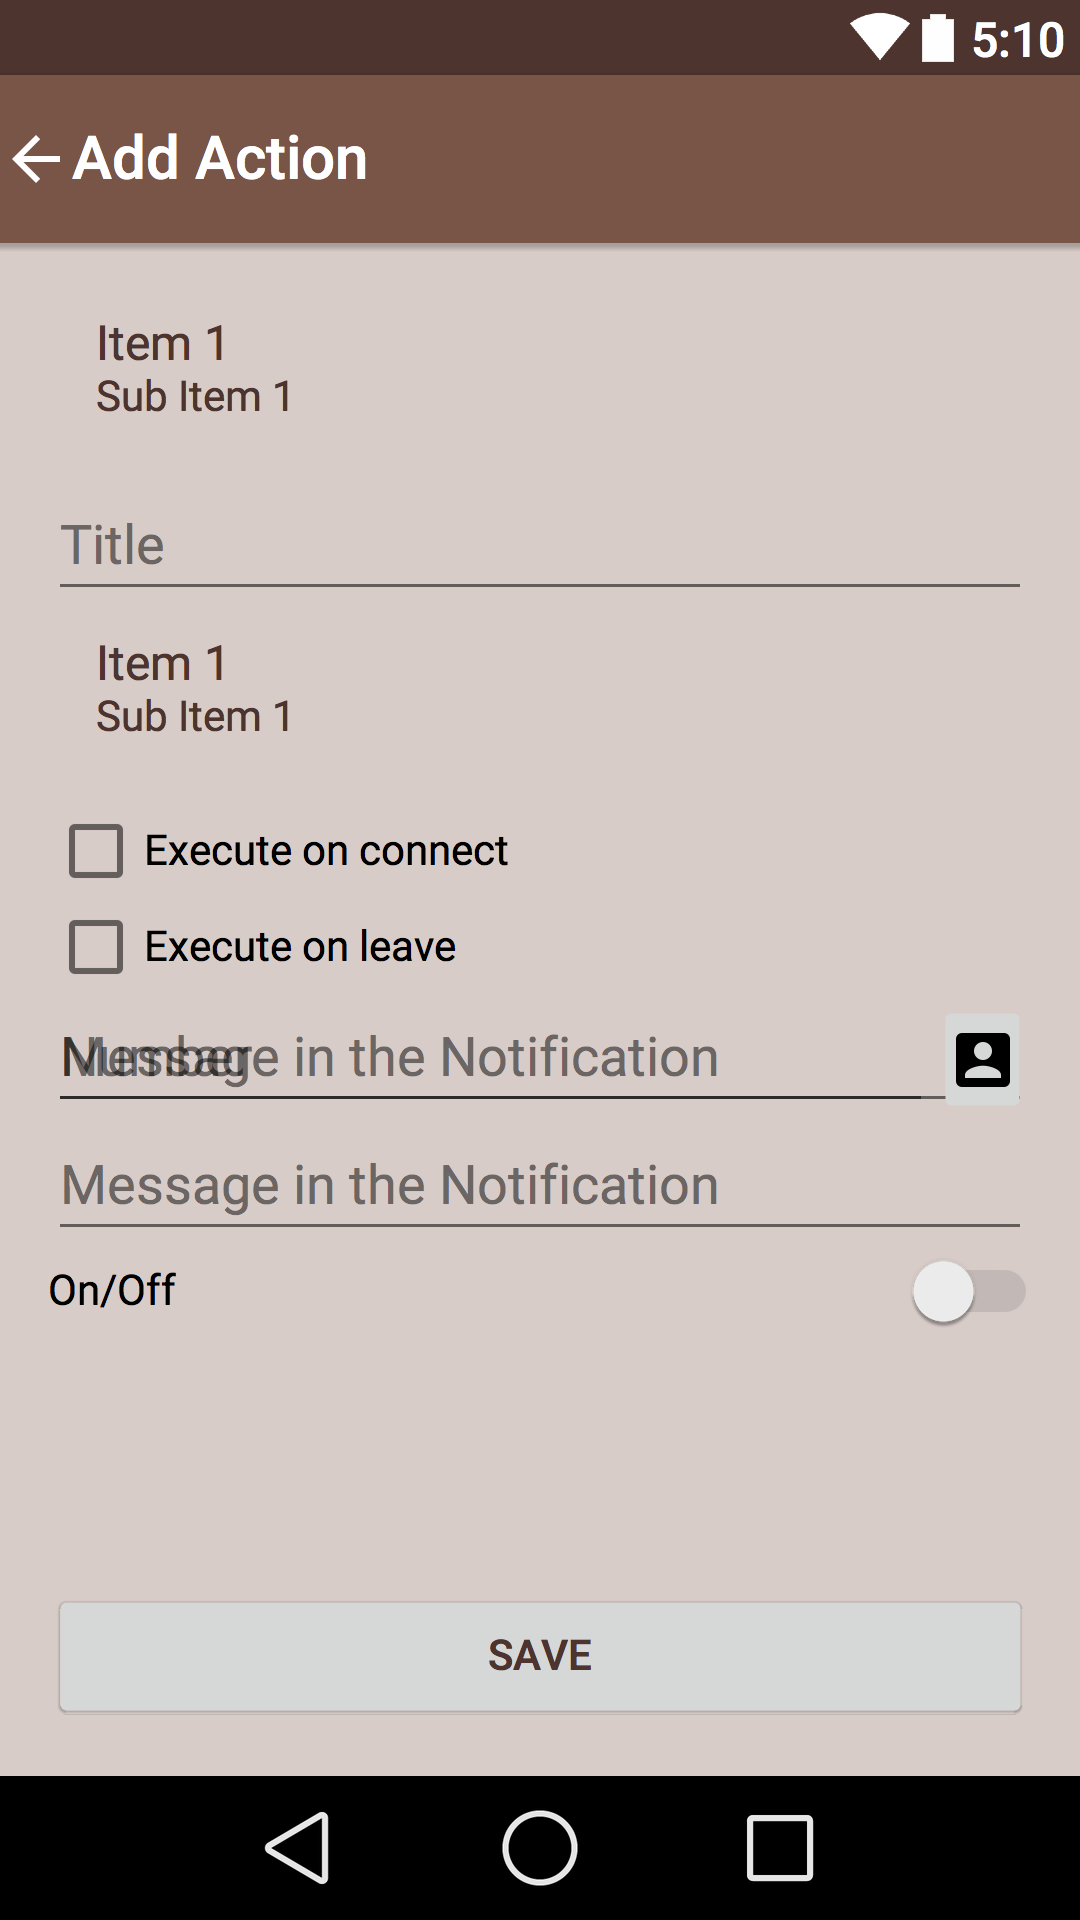
\includegraphics[width=0.4\textwidth]{images/actionactivity.png}
	\caption{Visuelle Repräsentation der ActionActivity}
	\label{fig:actionctivity}
\end{figure}

\subsubsection{LogActivity}
Die LogActivity ist im Vergleich zu den anderen Activities sehr schlicht. Aus einer Datenbank werden alle Log Einträge geladen und angezeigt. Der Adapter der ListView implementiert das ViewHolder Prinzip, welches auch bei sehr vielen Einträgen ein effizientes und für den Benutzer angenehmes Scrollen durch die Liste erlaubt.

% \begin{figure}[ht]
% 	\centering
% 	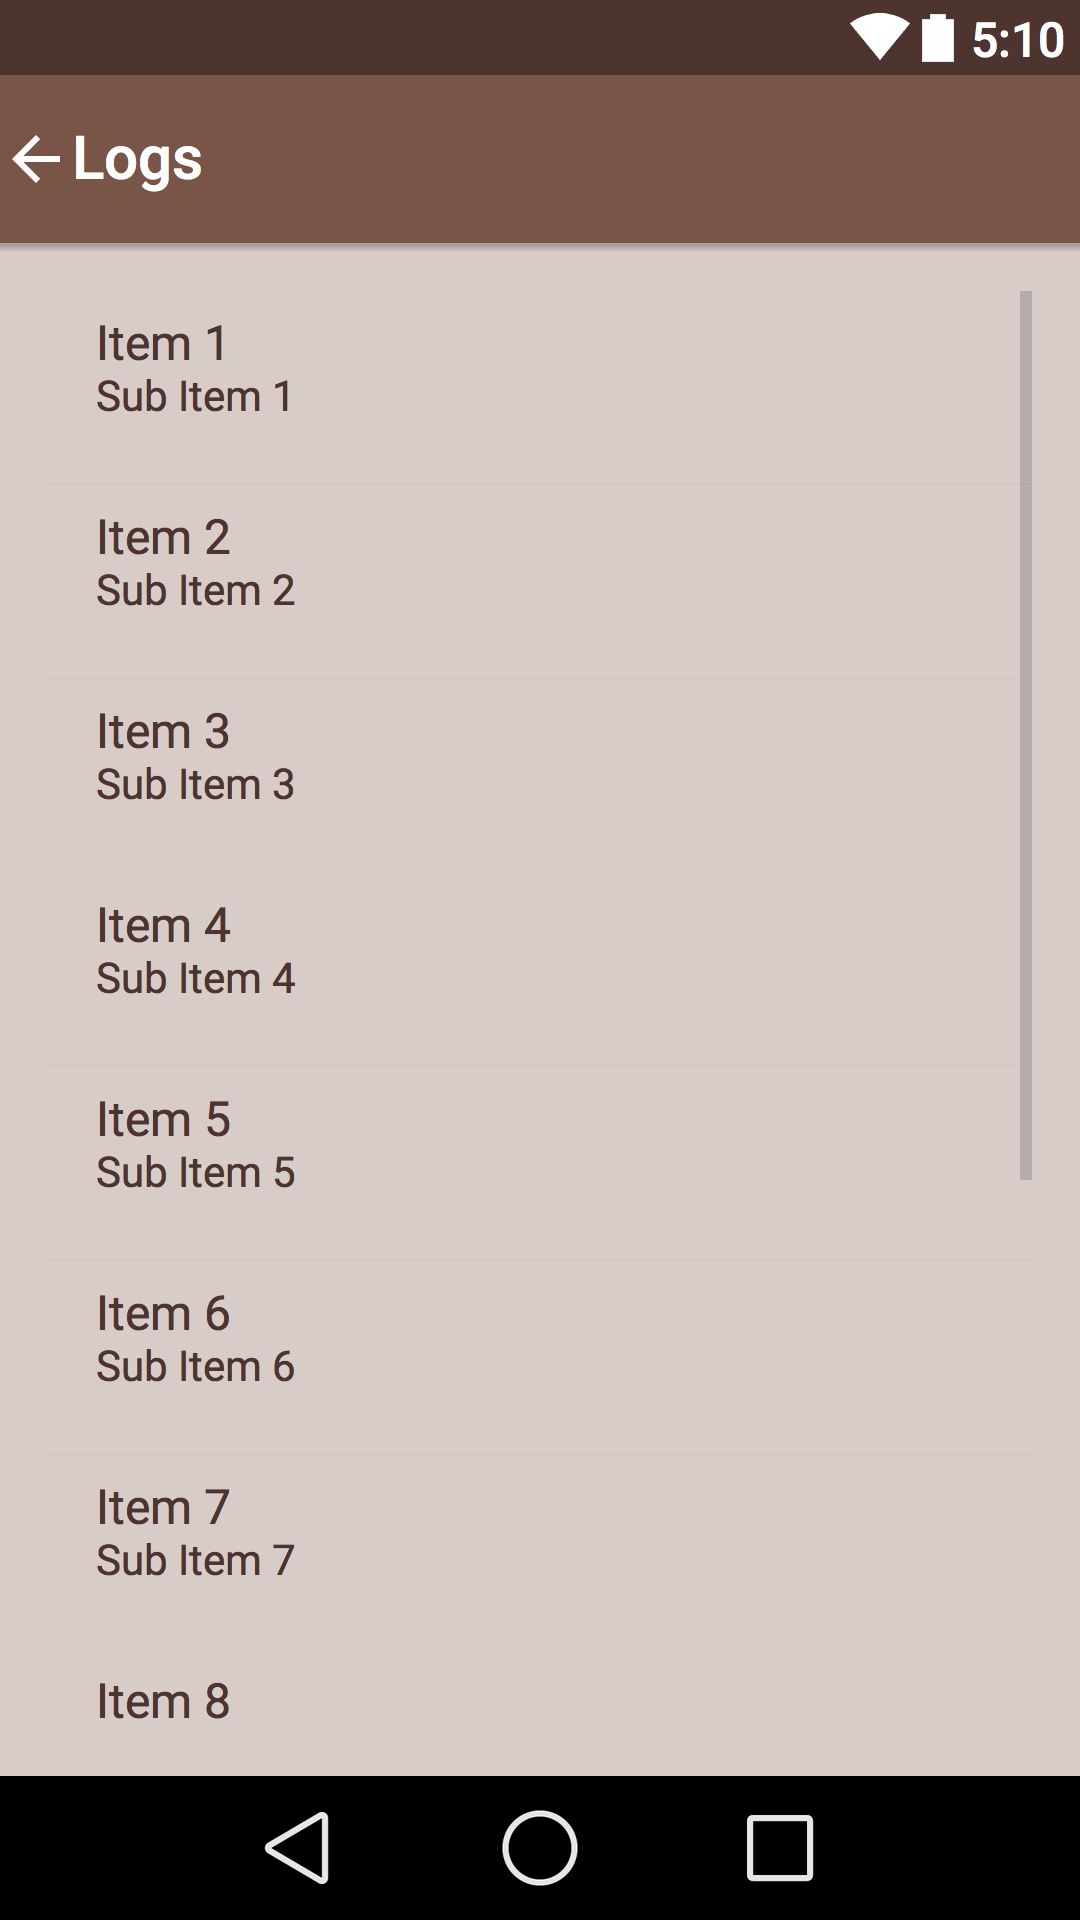
\includegraphics[width=0.4\textwidth]{images/logactivity.png}
% 	\caption{Visuelle Repräsentation der LogActivity}
% 	\label{fig:logactivity}
% \end{figure}

\newpage{}
\subsection{ConnectivityChangedReceiver}
Der ConnectivityChangedReceiver wird aktiviert und ausgeführt wenn es irgendeine Veränderung an der Netzwerkverbindung gibt. Diese Veränderung wird an den ActionService übergeben, welcher prüft ob eine Aktion ausgeführt werden muss. Dieser Ablauf ist im Sequenzdiagram in der Abbildung \ref{fig:seqactions} dargestellt.
\begin{figure}[ht]
    \centering
    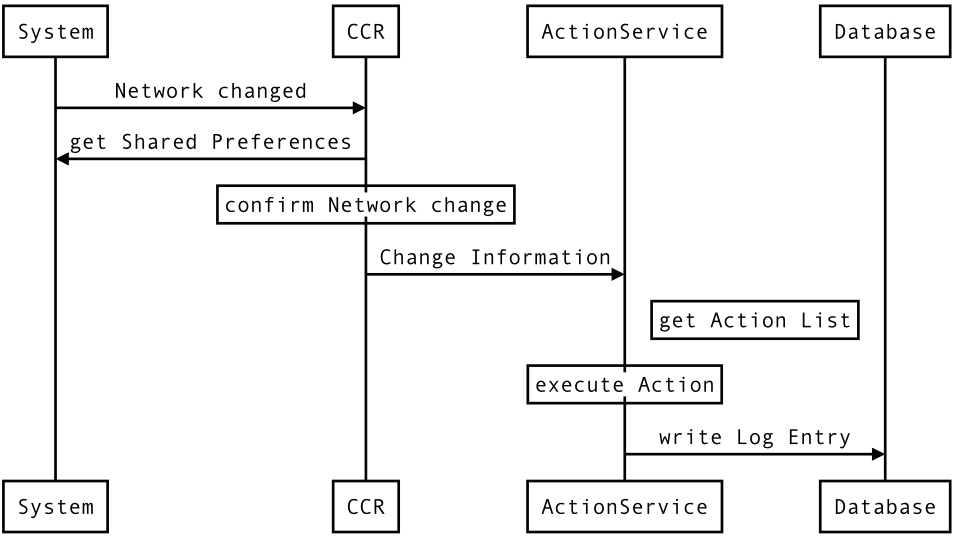
\includegraphics[width=0.8\textwidth]{images/seqActions.png}
    \caption{Sequenzdiagramm einer Netzwerkänderung}
    \label{fig:seqactions}
\end{figure}


 Der Receiver muss in der Lage sein zu wissen mit welchem Netzwerk das Mobiltelefon zuvor verbunden bzw. was der Status vor der Änderung der Netzwerkverbindung war. In einer ersten Implementation wurde dies mit Klassen Variabeln gelöst. Die Instanz des ConnectivityChangedReceiver lebt  aber nur während des Aufrufs und der Ausführung der onReceive Funktion. Darum ging der Wert der Variabeln nach kurzer Zeit Verloren. Die Lösung für dieses Problem heisst Shared Preferences. Mit den Shared Prefrences von Android können der Name und der Status der Netzwerkverbindung persistent gespeichert werden und bei der nächsten Ausführung von onReceive wieder gelesen werden. \\
\begin{lstlisting}[language=Java]
public void onReceive(Context context, Intent intent) {
    SharedPreferences sharedPreferences = context.getSharedPreferences("com.koki.app.wifiaction",Context.MODE_PRIVATE);
    String currentWifi = sharedPreferences.getString(CW,"");
    String currentState = sharedPreferences.getString(CS,"");
    ConnectivityManager cm = (ConnectivityManager) context.getSystemService(Context.CONNECTIVITY_SERVICE);
    NetworkInfo networkInfo = cm.getActiveNetworkInfo();
    if(networkInfo != null) {
        if(networkInfo.getTypeName().equals(currentState) && networkInfo.getExtraInfo().equals(currentWifi) ) {

        } else if (networkInfo.getTypeName().equals("WIFI") && !networkInfo.getExtraInfo().equals(currentWifi)) {
            ActionService.startAction(context, networkInfo.getExtraInfo(), true);
            sharedPreferences.edit().putString(CW, networkInfo.getExtraInfo()).putString(CS,networkInfo.getTypeName()).commit();
        } else if(currentState.equals("WIFI") && !networkInfo.getTypeName().equals("WIFI")) {
            ActionService.startAction(context, currentWifi, false);
            sharedPreferences.edit().putString(CW,networkInfo.getExtraInfo()).putString(CS,networkInfo.getTypeName()).commit();
        }
    }
}
\end{lstlisting}
In der Funktion onReceive wird überprüft ob der Verbindungstype gewechselt hat oder ob der Wireles LAN Netzwerkname geändert hat und die Funktion im ActionService mit den entsprechenden Parameter aufgerufen.

\subsection{ActionService}
Der ActionService erbt vom IntentService und wird beim Aufruf von onHandleIntent in einem eigenen Thread ausgeführt. Zuerst wird die Liste mit den Aktionen aus der Datei, welche die MainActivity schreibt, geladen. Danach wird überprüft ob für das aktuelle Wireless LAN und den Status der Verbindung eine Aktion existiert. Wird eine Aktion gefunden wird sie sogleich ausgeführt. Für jede Ausführung einer Aktion wird ein der Datenbank ein Log Eintrag erstellt. \\
\begin{lstlisting}[language=Java]
protected void onHandleIntent(Intent intent) {
    if (intent != null) {
        String wifi = intent.getStringExtra(EXTRA_WIFI);
        boolean isCon = intent.getBooleanExtra(EXTRA_ISCON,true);
        writeLog("WIFI CHANGE",wifi,isCon);
        ArrayList<Action> aList = loadFile();
        for(int i=0;i<aList.size();i++) {
            Action a = aList.get(i);
            if(a.getSsid().equals(wifi) && (a.isOnConnect() == isCon || a.isOnLeave() != isCon)) {
                switch(a.getActionType()) {
                    case BLUETOOTH:
                        handleActionBluetooth(a.isBooleanParam1());
                        break;
                    case GPS:
                        handleActionGPS(a.isBooleanParam1());
                        break;
                    case NOTIFICATION:
                        handleActionNotification(a.getStringParam1());
                        break;
                    case SMS:
                        handleActionSMS(a.getStringParam1(),a.getStringParam2());
                        break;
                }
                writeLog(a.getTitle(),wifi,isCon);
            }
        }
    }
}
\end{lstlisting}

\section{Restliche Implementationen}
Die Handhabung der Datenbank wurde mit einem neuen Framework namens Realm.io\footnote{Realm.io Mobile Database \url{http://realm.io/}} realisiert. Dieses Framework erleichtert das persistente Speichern sowie den Austausch von Daten zwischen verschiedenen Aktivitäten und Threads erheblich.
%!TEX root = ../doc.tex
\chapter{Fazit}
\label{sec:fazit}
Das Entwickeln eines Prototypen mit dem geplanten Funktionsumfang hat sich als machbar herausgestellt. Die App Funktioniert zuverlässig und kann von normalen Benutzern gebraucht werden. Die beiden Use Cases (UC-001 Aktion definieren und UC-002 Aktion ausführen) sowie die 6 Funktionalen Anforderungen, welche im Kapitel \ref{sec:anforderungsanalyse} beschrieben wurden, wurden alle umgesetzt. \newline{} Es hat sich jedoch herausgestellt dass das Anbieten von verschiedenen Aktionen schwieriger ist als ursprünglich angenommen. Das aktivieren bzw. deaktivieren des GPS Moduls ist auf einem Android Mobiltelefon ohne Interaktion eines Benutzers nicht möglich. Auch für eine Aktion, welche es erlaubt eine Email zu verschicken muss bedeutend mehr Programmiert werden. Zum Beispiel müssen die aktiven Benutzerkonten geladen werden wofür wieder mehr Berechtigungen benötigt werden. Aber es gibt auch kleinere Verbesserungen welche noch nicht implementiert sind. So sollten die Aktionen auch in der Datenbank gespeichert werden anstatt in eine Datei serialisiert zu werden. Für die besser Stabilität sollten Tests definiert werden und vor einer Veröffentlichung sollte die App auf mehreren Geräten getestet werden. Das Projekt wird nach Abgabe dieser Seminararbeit weiter verfolgt werden.



%\chapter{Verzeichnisse}
%\label{sec:Verzeichnisse}
\addcontentsline{toc}{chapter}{Verzeichnisse}
\addcontentsline{toc}{section}{Literaturverzeichnis}
\bibliography{BibTeX/literatur}
\listoffigures
\addcontentsline{toc}{section}{Abbildungsverzeichnis}
%\listoftables
%\addcontentsline{toc}{section}{Tabellenverzeichnis}
%%!TEX root = ../doc.tex
\chapter*{Glossar}
\label{sec:Glossar}
\addcontentsline{toc}{section}{Abkürzungsverzeichnis}\label{cha:abkürzungsverzeichnis}

In diesem Abschnitt werden Abkürzungen und Begriffe kurz erklärt.
\setglossarystyle{altlistgroup}
\printglossary[title=]


%\lstlistoflistings
%\addcontentsline{toc}{section}{Listingverzeichnis}

%%!TEX root = ../doc.tex
\pagenumbering{Roman}

\appendix
\chapter{Anhang}
\label{sec:Anhang}

\section{Projektmanagement}\label{projektmanagement}

\textcolor{darkgray}{
  \begin{itemize}
  \item Offizielle Aufgabenstellung, Projektauftrag
  \item (Zeitplan)
  \item (Besprechungsprotokolle oder Journals)
  \end{itemize}
}

\section{Weiteres}
\label{sec:Weiteres}

\textcolor{darkgray}{
  \begin{itemize}
  \item CD mit dem vollständigen Bericht als pdf-File inklusive Film- und Fotomaterial
  \item (Schaltpläne und Ablaufschemata)
  \item (Spezifikationen u. Datenblätter der verwendeten Messgeräte und/oder Komponenten)
  \item (Berechnungen, Messwerte, Simulationsresultate)
  \item (Stoffdaten)
  \item (Fehlerrechnungen mit Messunsicherheiten)
  \item (Grafische Darstellungen, Fotos)
  \item (Datenträger mit weiteren Daten (z.B. Software-Komponenten) inkl. Verzeichnis der auf diesem Datenträger abgelegten Dateien)
  \item (Softwarecode)
  \end{itemize}
}


\end{document}
